\documentclass{article}

\usepackage{graphicx}
\usepackage{tikz}
\usepackage{tikzsymbols}
\usetikzlibrary{calc,patterns,shapes.geometric}
\pagestyle{empty}
\usepackage[margin=0pt]{geometry}
\geometry{papersize={14in,12in}}

\def\centerarc[#1](#2)(#3:#4:#5){\draw[#1] ($(#2)+({#5*cos(#3)},{#5*sin(#3)})$) arc (#3:#4:#5);}

\begin{document}
	\begin{figure}
		\centering
		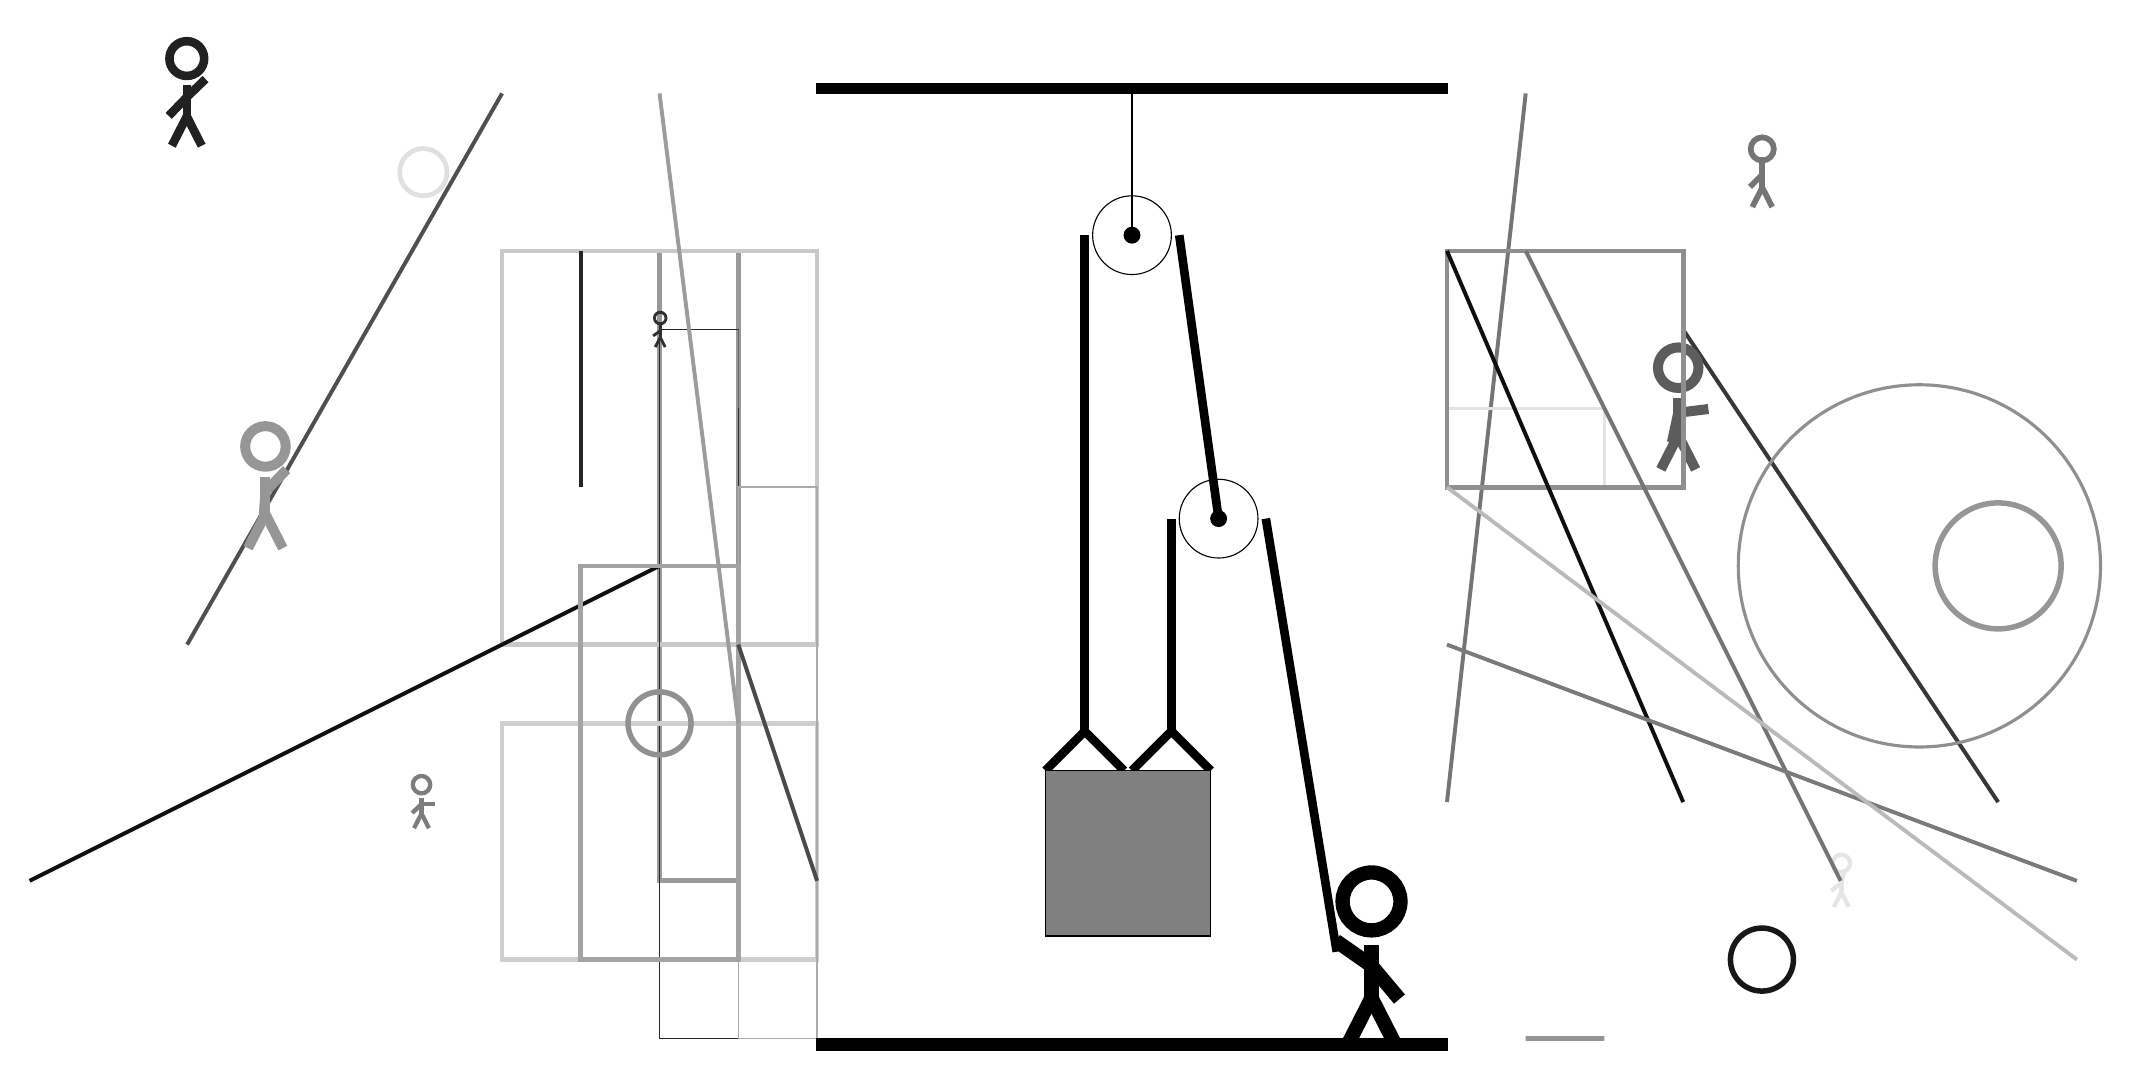
\begin{tikzpicture}
			%%%%% START %%%%%
			
			\draw[fill=black] (-2, 9) rectangle (6, 9.125);
			
			\draw (2, 7.2) circle (0.5);
			\draw[fill=black] (2, 7.2) circle (0.1);
			\draw[thick] (2, 7.2) -- (2, 9);
			
			\draw (3.1, 3.6) circle (0.5);
			\draw[fill=black] (3.1, 3.6) circle (0.1);
			
			\node[line width=0.6mm, color=black!51] at (-7, 0) {\Strichmaxerl[3][44][0]};
			
			\draw[line width=0.5mm, color=black!54](6, 0) -- (7, 9);
			\draw[line width=0.5mm, color=black!78](9, 6) -- (13, 0);
			\draw[line width=0.3mm, color=black!11] (6, 4) rectangle (8, 5);
			\draw[line width=0.6mm, color=black!40] (-4, -1) rectangle (-3, 7);
			\draw[line width=0.6mm, color=black!21] (-2, 2) rectangle (-6, 7);
			
			\draw[line width=0.5mm, color=black!85](-5, 4) -- (-5, 7);
			\node[line width=0.5mm, color=black!10] at (11, -1) {\Strichmaxerl[3][39][76]};
			\node[line width=0.4mm, color=black!54] at (10, 8) {\Strichmaxerl[4][45][90]};
			\draw[line width=0.2mm, color=black!84] (-4, -3) rectangle (-3, 6);
			\draw[line width=0.6mm, color=black!19] (-2, -2) rectangle (-6, 1);
			\node[line width=0.3mm, color=black!87] at (-10, 9) {\Strichmaxerl[6][46][44]};
			\node[line width=0.6mm, color=black!64] at (9, 5) {\Strichmaxerl[7][78][7]};
			
			\draw[line width=0.5mm, color=black!94](-4, 3) -- (-12, -1);
			\draw[line width=0.5mm, color=black!69](-6, 9) -- (-10, 2);
			\draw [line width=0.4mm, color=black!44](12, 3) circle (2.3);
			
			\draw[line width=0.6mm, color=black!44] (6, 4) rectangle (9, 7);
			
			\draw[line width=0.5mm, color=black!54](11, -1) -- (7, 7);
			\draw[line width=0.5mm, color=black!94](6, 7) -- (9, 0);
			\draw [line width=0.6mm, color=black!12](-7, 8) circle (0.3);
			\node[line width=0.6mm, color=black!41] at (-9, 4) {\Strichmaxerl[7][86][46]};
			
			\draw [line width=0.7mm, color=black!43](-4, 1) circle (0.4);
			\draw[line width=0.2mm, color=black!61] (-3, 6) rectangle (-3, 5);
			\draw[line width=0.2mm, color=black!33] (-3, 4) rectangle (-2, -3);
			\draw[line width=0.5mm, color=black!52](6, 2) -- (14, -1);
			
			\node[line width=0.2mm, color=black!81] at (-4, 6) {\Strichmaxerl[2][35][88]};
			
			\draw [line width=0.7mm, color=black!41](13, 3) circle (0.8);
			\draw [line width=0.7mm, color=black!91](10, -2) circle (0.4);
			\draw[line width=0.6mm, color=black!36] (-3, 3) rectangle (-5, -2);
			\draw[line width=0.5mm, color=black!27](6, 4) -- (14, -2);
			\draw[line width=0.7mm, color=black!42] (8, -3) rectangle (7, -3);
			\draw[line width=0.5mm, color=black!71](-2, -1) -- (-3, 2);
			\draw[line width=0.5mm, color=black!39](-4, 9) -- (-3, 1);
			
			\draw[line width = 1.1mm]  (0.9, 0.4) -- (1.4, 0.9) -- (1.9, 0.4);
			\draw[line width = 1.1mm]  (2.0, 0.4) -- (2.5, 0.9) -- (3.0, 0.4);
			\draw[fill=black!50] (0.9, 0.4) rectangle (3.0, -1.7);
			
			\draw[line width = 1.1mm] (1.4, 7.2) -- (1.4, 0.9);
			\centerarc[line width = 1.1mm](2, 7.2)(0:180:0.6);
			\draw[line width = 1.1mm] (2.6, 7.2) -- (3.1, 3.6);
			\draw[line width = 1.1mm] (2.5, 3.6) -- (2.5, 0.9);
			\centerarc[line width = 1.1mm](3.1, 3.6)(0:180:0.6);
			\draw[line width = 1.1mm] (3.7, 3.6) -- (4.6, -1.9);
			
			\node at (5, -2) {\Strichmaxerl[10][-35][-50]};
			
			\draw[fill=black] (-2, -3) rectangle (6, -3.15);
			
			%%%%% END %%%%%
		\end{tikzpicture}
	\end{figure}	
\end{document}